\documentclass{article}

\usepackage{arxiv}

\usepackage[utf8]{inputenc}
\usepackage[T1]{fontenc}
\usepackage[hidelinks]{hyperref}
\usepackage{url}
\usepackage{booktabs}
\usepackage{amsmath}
\usepackage{amsfonts}
\usepackage{amssymb}
\usepackage{microtype}
\usepackage{graphicx}
\usepackage{natbib}
\usepackage{caption}
\captionsetup{font=footnotesize,labelfont=bf,justification=justified,singlelinecheck=false}
\captionsetup[table]{skip=4pt}
\captionsetup[figure]{skip=6pt}
\usepackage{needspace}
\usepackage{multicol}
\bibliographystyle{unsrtnat}

%% ---- page layout -------------------------------------------------------
%% A section heading never appears at the bottom of a page: if less than a
%% quarter of the page is left, the section starts at the top of the next one.
%% Pages are vertically justified (\flushbottom) so no page ends ragged, and
%% the float parameters let tables and figures pack tightly with the text
%% instead of drifting onto pages of their own.
%% tighter page: slightly larger text block and less vertical air than the
%% stock template, so the report fits its page budget without shrinking type.
\AtBeginDocument{\newgeometry{textheight=9.3in,textwidth=6.9in,top=0.9in,
  headheight=14pt,headsep=16pt,footskip=24pt}}
\setlength{\parskip}{1.5pt plus 1pt minus 1pt}
\setlength{\textfloatsep}{9pt plus 3pt minus 2pt}
\setlength{\intextsep}{9pt plus 3pt minus 2pt}
\setlength{\abovecaptionskip}{3pt}
\setlength{\belowcaptionskip}{2pt}
\flushbottom
\setcounter{topnumber}{3}
\setcounter{bottomnumber}{2}
\setcounter{totalnumber}{4}
\renewcommand{\topfraction}{0.92}
\renewcommand{\bottomfraction}{0.60}
\renewcommand{\textfraction}{0.06}
\renewcommand{\floatpagefraction}{0.60}
\newif\iffirstsectiondone
\let\originalsection\section
\renewcommand{\section}{%
  \iffirstsectiondone\Needspace*{0.12\textheight}\else\firstsectiondonetrue\fi
  \originalsection}
\setlength{\bibsep}{1pt}
\newcommand{\numWords}{34}
\newcommand{\numCompare}{3{,}297}
\newcommand{\numEarlier}{3{,}400}
\newcommand{\numLater}{3{,}400}
\newcommand{\numTotalPairs}{10{,}097}
\newcommand{\numUses}{6{,}594}
\newcommand{\bestLayer}{5}
\newcommand{\zsF}{63.6}
\newcommand{\zsOracleF}{70.3}
\newcommand{\zsOracleLayer}{8}
\newcommand{\lastLayerF}{68.0}
\newcommand{\jaccardF}{53.5}
\newcommand{\randomF}{50.6}
\newcommand{\ftF}{61.9}
\newcommand{\ftFsd}{1.4}
\newcommand{\ftVal}{66.3}
\newcommand{\numSeeds}{3}
\newcommand{\simlrF}{65.4}
\newcommand{\mainModelVal}{75.7}
\newcommand{\mainModel}{cos L5}
\newcommand{\rhoCompare}{-0.61}
\newcommand{\rhoCompareP}{0.0001}
\newcommand{\rhoDeltaCompare}{-0.23}
\newcommand{\rhoDeltaCompareP}{0.1859}
\newcommand{\rhoDeltaLater}{0.34}
\newcommand{\rhoDeltaLaterP}{0.0484}
\newcommand{\goldAgree}{0.33}
\newcommand{\nReductive}{31}
\newcommand{\nInnovative}{3}
\newcommand{\hardestWord}{bullpen}
\newcommand{\hardestAcc}{42.4}
\newcommand{\easiestWord}{delta}
\newcommand{\easiestAcc}{86.7}
\newcommand{\nBelowMajority}{11}
\newcommand{\nTestWords}{15}
\newcommand{\rhoBalanceAcc}{0.60}
\newcommand{\rhoBalanceAccP}{0.017}


\title{Usage Relatedness for English Social Media:\\
Transferring the DURel Framework to TempoWiC}

\author{
  Raja Kishore Reddy Talakola \\
  Matriculation Number: 1866163 \\
}

\renewcommand{\headeright}{Replication Report}
\renewcommand{\undertitle}{Replication and extension of \citet{schlechtweg2018durel}}

\date{September 2026}

\begin{document}
\maketitle

\begin{abstract}
\citet{schlechtweg2018durel} propose DURel, a framework for annotating
\emph{Diachronic Usage Relatedness}, and apply it to German historical text
(DTA). Their study produced a test set of 1{,}320 use pairs for 22 target words.
This report runs the same framework on English instead of German. The corpus is
\textbf{TempoWiC} \citep{loureiro2022tempowic}, an English Twitter benchmark in
which two tweets from different years are labelled for whether a target word
carries the same meaning. TempoWiC only contains cross-period pairs, so we
rebuild the missing within-period pairs by sampling from the same tweets. The
result is \numTotalPairs{} use pairs for \numWords{} target words in DURel's
three groups: EARLIER, LATER and COMPARE. Human annotators are replaced by
relatedness models, from lexical overlap to a fine-tuned cross-encoder. On the
TempoWiC task, zero-shot target-word cosine reaches
\zsF{} macro-F1 and supervised training does not improve on it
(\ftF{}\,$\pm$\,\ftFsd{} for the cross-encoder), because the training and test
splits share no target words. At the word level, COMPARE correlates with the
human change rate at $\rho=\rhoCompare$ ($p=\rhoCompareP$), which supports the
original claim that COMPARE measures the \emph{degree} of change. $\Delta$LATER
does not transfer. On 2019--2021 Twitter data it mostly reflects pandemic
vocabulary, which makes later usage more homogeneous rather than less. The code,
the data pipeline and all result files are released with this report.
\end{abstract}

\section{Introduction}

Work on lexical semantic change is limited more by evaluation data than by
models \citep{schlechtweg2018durel}. DURel addresses this by moving
\emph{synchronic} polysemy annotation into a diachronic setting. Annotators
never see a sense inventory. They only judge how related two \emph{uses} of a
word are, on a four-point scale, and change is read off the resulting means. The
original study is German, historical (DTA, 1750--1800 vs.\ 1850--1900) and
annotated by people.

This report asks one question: does that design still work in English, on social
media, over a two-year gap instead of a century, with models doing the rating?
We use TempoWiC \citep{loureiro2022tempowic}, which is built from tweets sampled
one year apart and already carries human labels. Those labels give us something
the German study did not have, namely an independent measurement of how much
each word changed.

The report contributes three things: a DURel-style dataset for English social
media (\numTotalPairs{} use pairs for \numWords{} target words in three groups,
rebuilt from TempoWiC, \S\ref{sec:design}); relatedness models used in place of
annotators, evaluated on the original TempoWiC task and put through an agreement
analysis in the shape of DURel's Table~3 (\S\ref{sec:pairwise},
\S\ref{sec:agreement}); and a numerical test of both DURel change measures
against human judgements, which the German study could not run
(\S\ref{sec:measures}).

\section{Related work}
\label{sec:related}

\paragraph{Annotating meaning in context.} Judging pairs of \emph{uses} rather
than assigning senses from an inventory goes back to synchronic work on graded
polysemy. \citet{brown2008choosing} asks annotators how fine-grained sense
distinctions really are, and \citet{erk2013measuring} show that annotators can
rate word meaning in context reliably on a graded scale, with average pairwise
correlations between $0.55$ and $0.62$. DURel \citep{schlechtweg2018durel} takes
that idea into the diachronic setting, which is the framework this report
applies. The same line of work later scaled up into Word Usage Graphs: DWUG
\citep{schlechtweg2021dwug} collects around 100{,}000 human proximity judgements
in four languages and clusters uses into senses instead of reading change off
group means. Our study sits between the two. We keep DURel's simple group means,
but we obtain the judgements from models rather than from people.

\paragraph{Benchmarks.} Two benchmark families are relevant. The first evaluates
change at the level of the word: SemEval-2020 Task~1
\citep{schlechtweg2020semeval} asks systems to decide whether a target word lost
or gained a sense between two corpora in English, German, Latin and Swedish, with
gold data built from the annotation procedure above. The second evaluates
meaning at the level of the pair: WiC \citep{pilehvar2019wic} asks whether a
target word carries the same meaning in two contexts, and TempoWiC
\citep{loureiro2022tempowic} is its diachronic, social-media version, where the
two contexts are tweets from different years. TempoWiC is the corpus we use.
Its pair-level labels are what let us test DURel's word-level measures against
an independent human measurement, which neither benchmark family does on its
own.

\paragraph{Computational models of change.} Early work compares static
embedding spaces trained per period and aligns them
\citep{hamilton2016cultural}; \citet{kutuzov2018survey} survey that generation of
methods. Contextualised encoders changed the picture, since a word no longer has
one vector per period but one per use. \citet{giulianelli2020analysing} cluster
contextual representations of individual uses and derive change measures from
how those clusters move, which is close in spirit to DURel's use pairs.
\citet{loureiro2022timelms} take the other route and pre-train Twitter encoders
per time period (TimeLMs); those models provide the strongest baselines in the
TempoWiC shared task. Our relatedness models belong to the contextual-encoder
family, without the time-specific pre-training, for the reason given in
\S\ref{sec:setup}.

\paragraph{Models as annotators.} Using a model where an annotation study would
use people is now common, and it is what makes a study of this size possible
without an annotation budget. The practice has a known cost: a model's
judgements are correlated with its own training data and architecture, so a
panel of models is not a panel of independent raters.
\S\ref{sec:agreement} quantifies that cost on our data by putting the models
through exactly the agreement analysis the German study ran on its five
annotators. Table~\ref{tab:resources} places this report next to the resources
it borrows from.

\begin{table}[t]\centering\footnotesize
\caption{Resources for meaning change and meaning in context. The unit judged is
what a single annotation decision covers.}
\label{tab:resources}
\begin{tabular}{@{}lllll@{}}
\toprule
Resource & Languages & Genre & Unit judged & Size \\
\midrule
DURel \citep{schlechtweg2018durel} & German & historical prose & use pair, 1--4 & 1{,}320 pairs \\
DWUG \citep{schlechtweg2021dwug} & 4 languages & mixed historical & use pair, 1--4 & $\sim$100k judgements \\
SemEval-2020 T1 \citep{schlechtweg2020semeval} & 4 languages & historical corpora & word, binary + rank & 137 words \\
WiC \citep{pilehvar2019wic} & English & dictionary examples & use pair, binary & 7{,}466 pairs \\
TempoWiC \citep{loureiro2022tempowic} & English & tweets & use pair, binary & 3{,}297 pairs \\
\midrule
This report & English & tweets & use pair, 1--4 (model) & 10{,}097 pairs \\
\bottomrule
\end{tabular}
\end{table}

\paragraph{Position of this report.} The contribution is not a new model. It is a
transfer of an annotation framework to a new language, genre and time scale, plus
the first numerical check of its two change measures against human judgements of
change.

\section{Background}

\paragraph{DURel.} A \emph{use} of a word is the sentence it occurs in. Uses are
shown in pairs and rated 1 (\textit{Unrelated}), 2 (\textit{Distantly related}),
3 (\textit{Closely related}) or 4 (\textit{Identical}); 0 means ``cannot
decide''. Pairs come from three groups: EARLIER (both uses from $t_1$), LATER
(both from $t_2$) and COMPARE (one from each). Two measures follow from the
group means:
\begin{align}
\Delta\textsc{later}(w) &= \mathrm{Mean}_l(w) - \mathrm{Mean}_e(w) \\
\textsc{compare}(w) &= \mathrm{Mean}_c(w)
\end{align}
A negative $\Delta$LATER means \emph{innovative} change: a new meaning appears,
so later pairs are less related. A positive value means \emph{reductive} change,
where a meaning is lost. COMPARE measures the degree of change and does not
distinguish the two types. The paper also proposes a polysemy-normalised
variant, $\Delta\textsc{compare}(w)=\mathrm{Mean}_c(w)-\mathrm{Mean}_e(w)$.

Table~\ref{tab:scale} gives the rating scale, and Figure~\ref{fig:schematic}
shows how the three groups are formed. The design has one property that matters
for everything below: a rater never has to name a sense, and never has to know
that the study is about change at all. All the diachronic information sits in
which group a pair was drawn from.

\begin{table}[t]\centering\small
\caption{The four-point relatedness scale used by DURel, after
\citet{brown2008choosing}. Our models produce scores on this scale by the
mapping in \S\ref{sec:models}.}
\label{tab:scale}
\begin{tabular}{@{}cll@{}}
\toprule
Score & Label & Reading \\
\midrule
4 & Identical & the two uses carry the same meaning \\
3 & Closely related & the same meaning, used in different contexts \\
2 & Distantly related & related meanings, e.g.\ literal vs.\ figurative \\
1 & Unrelated & homonymy: no shared meaning \\
0 & Cannot decide & rater abstains (excluded from the means) \\
\bottomrule
\end{tabular}
\end{table}

\begin{figure}[t]\centering
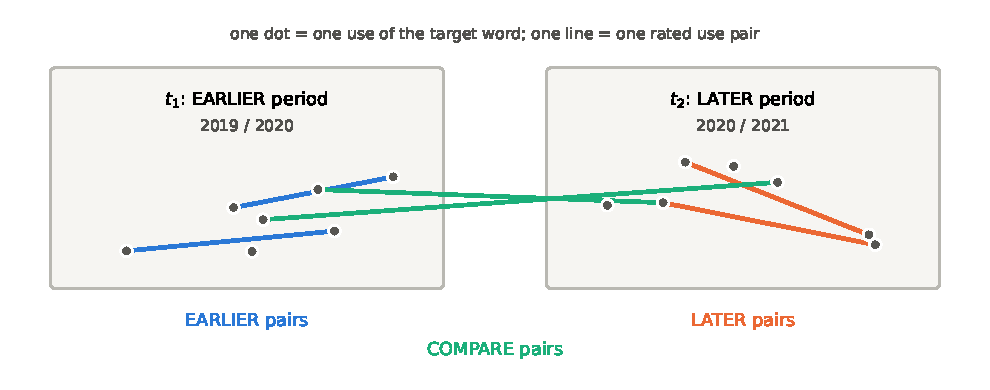
\includegraphics[width=0.66\linewidth]{../figures/fig_groups_schematic.pdf}
\caption{The three groups of use pairs. EARLIER and LATER pairs measure how
homogeneous a single period is; COMPARE pairs measure the two periods against
each other.}
\label{fig:schematic}
\end{figure}

\paragraph{TempoWiC.} TempoWiC \citep{loureiro2022tempowic} is the dataset of the
EvoNLP 2022 shared task. One instance is a target word with two tweets, one per
time period, and a binary label: \emph{same meaning} or \emph{different
meaning}. The tweets are tokenised, the character span of the target is given,
and every tweet carries a \texttt{YYYY-MM} date. Gold test labels were released
in 2023. Table~\ref{tab:example} shows two real instances for \textit{frisk},
one of each label: both pairs share little vocabulary, and only the meaning of
the target separates them.

\begin{table}[t]\centering\small
\caption{Two TempoWiC training instances for the target word \textit{frisk}
(target in bold). The second pair contrasts the game character with the
stop-and-frisk policy.}
\label{tab:example}
\begin{tabular}{@{}l p{0.80\linewidth}@{}}
\toprule
\multicolumn{2}{@{}l}{Target word: \textit{frisk}} \\
\midrule
2019-02 & Also, just for the record, LabCorp in Frederick all but does a \textbf{frisk} search before your piss test. \\
2020-02 & why did my AFRICAN dad just say that Bloomberg's stop and \textbf{frisk} was good for New York? \\
\multicolumn{2}{r}{\textit{gold label: same meaning}} \\
\midrule
2019-02 & new one wut is \textbf{frisk} \\
2020-02 & The stop and \textbf{frisk} guy is now endorsing the crime bill guy in the most shocking turn of events \\
\multicolumn{2}{r}{\textit{gold label: different meaning}} \\
\bottomrule
\end{tabular}
\end{table}

\section{Adapting DURel to TempoWiC}
\label{sec:design}

\subsection{How this study lines up with the original}

Table~\ref{tab:alignment} states the correspondence between the German study and
this one, element by element. Everything in the left column is kept; only the
material it is applied to changes. Three cells are genuine departures and are
discussed where they matter: the annotators (\S\ref{sec:agreement}), the
within-period pairs, which TempoWiC does not supply and we sample
(\S\ref{sec:groups}), and the validation of the measures, which we can do
numerically (\S\ref{sec:measures}).

\begin{table}[t]\centering\footnotesize
\caption{Alignment between \citet{schlechtweg2018durel} and this report. Rows
marked $\dagger$ are where the two studies differ by necessity rather than by
choice.}
\label{tab:alignment}
\begin{tabular}{@{}lll@{}}
\toprule
Element & \citet{schlechtweg2018durel} & This report \\
\midrule
Corpus & DTA, German historical prose & TempoWiC, English tweets \\
Time periods & 1750--1800 vs.\ 1850--1900 & year $Y$ vs.\ $Y{+}1$ (2019--2021) \\
Definition of a use & sentence, with neighbouring sentences & one tweet \\
Target words & 22 & 34 \\
Use pairs & 1{,}320 & 10{,}097 \\
Pairs per word and group & 20 & 100 (EARLIER / LATER) \\
Groups & EARLIER, LATER, COMPARE & identical \\
Relatedness scale & 1--4, 0 = cannot decide & 1--4, mapped from model scores \\
Raters$^\dagger$ & 5 human annotators & 5 relatedness models \\
Within-period pairs$^\dagger$ & sampled from the corpus & sampled from TempoWiC's tweets \\
Agreement analysis & pairwise Spearman between raters & identical, plus vs.\ gold labels \\
Change measures & $\Delta$LATER, COMPARE, $\Delta$COMPARE & identical \\
Validation of measures$^\dagger$ & qualitative, historical dictionaries & numerical, vs.\ human change rate \\
\bottomrule
\end{tabular}
\end{table}

\subsection{Target words and periods}

We use all \numWords{} target words from the train, validation and test splits.
For every word, TempoWiC pairs a tweet from month $m$ of year $Y$ with a tweet
from month $m$ of year $Y{+}1$. We take year $Y$ as $t_1$ and year $Y{+}1$ as
$t_2$ (Table~\ref{tab:data}). The gap is therefore one year, against the century
between DTA's two periods. This is in line with the original recommendation to
use directly adjacent and short time periods.

\begin{table}[t]\centering\small
\caption{TempoWiC splits as used here. Only gold-labelled test instances are
kept; the dummy instances in the released test file are discarded.}
\label{tab:data}
\begin{tabular}{lrrrrc}
\toprule
Split & Words & COMPARE pairs & same & different & $t_1$/$t_2$ \\
\midrule
Train & 15 & 1{,}428 & 650 & 778 & 2019/2020 \\
Validation & 4 & 396 & 172 & 224 & 2019/2020 \\
Test & 15 & 1{,}473 & 539 & 934 & 2020/2021 \\
\midrule
All & 34 & 3{,}297 & 1{,}361 & 1{,}936 & -- \\
\bottomrule
\end{tabular}
\end{table}

\subsection{Rebuilding the three groups}
\label{sec:groups}

Every TempoWiC instance is a COMPARE pair by construction. EARLIER and LATER
pairs do not exist in the benchmark, so we sample them from the same tweets. For
each word we collect all unique uses inside one period and draw 100 distinct
pairs per word and period at random (seed 42). As in DURel, no use pair is
sampled twice within a group. Table~\ref{tab:groups} gives the result:
\numEarlier{} EARLIER pairs, \numLater{} LATER pairs and \numCompare{} COMPARE
pairs over \numUses{} unique uses.

\begin{table}[t]\centering\small
\caption{Use pairs per DURel group.}
\label{tab:groups}
\begin{tabular}{lrl}
\toprule
Group & Use pairs & Source \\
\midrule
EARLIER ($t_1$,$t_1$) & 3{,}400 & sampled (100 per word) \\
LATER ($t_2$,$t_2$) & 3{,}400 & sampled (100 per word) \\
COMPARE ($t_1$,$t_2$) & 3{,}297 & original TempoWiC pairs (gold-labelled) \\
\midrule
Total & 10{,}097 & \\
\bottomrule
\end{tabular}
\end{table}

\subsection{Sampling and sanity checks}

Table~\ref{tab:useinventory} summarises what is available per word. A word has
between 76 and 100 unique uses per period, which is enough for 100 distinct
within-period pairs but not enough for every pair to use a distinct tweet, so a
single use may appear in more than one pair. DURel allows exactly this when the
pool is small.

\texttt{src/verify.py} checks three properties of the construction, all of which
hold: no use pair occurs twice inside a group, no EARLIER or LATER pair mixes the
two years, and no COMPARE pair sits inside one year. Uses are deduplicated by
tweet text plus the target's character span, so one tweet is never two uses.

\begin{table}[t]\centering\small
\caption{Inventory per target word.}
\label{tab:useinventory}
\begin{tabular}{@{}lrrr@{}}
\toprule
Per target word & min & median & max \\
\midrule
Unique uses in $t_1$ & 76 & 98 & 100 \\
Unique uses in $t_2$ & 76 & 98 & 100 \\
COMPARE pairs (gold) & 76 & 98 & 100 \\
EARLIER / LATER pairs sampled & 100 & 100 & 100 \\
\bottomrule
\end{tabular}
\end{table}

\subsection{Models instead of annotators}
\label{sec:models}

DURel's five students are replaced by five relatedness models, each mapping a
use pair to a graded relatedness score. \textbf{Jaccard} is the content-word
overlap of the two tweets, a purely lexical control. \textbf{Sentence cosine} is
the cosine between the mean-pooled tweet vectors. \textbf{Target cosine} is the
cosine between the contextual vectors of the target word itself at encoder layer
$k$, where the target vector is the mean over its sub-word pieces and the layer
is selected on the validation split. \textbf{Similarity logistic regression} is
trained on the training split over all 15 similarity features (13 layer cosines,
sentence cosine, Jaccard), the same family as the strongest official shared-task
baseline. The \textbf{fine-tuned cross-encoder} is trained on the same split.

Scores are mapped onto DURel's 1--4 scale. For the classifiers we use
$\mathrm{rel}=1+3\hat{p}$, where $\hat{p}$ is the probability of \emph{same
meaning}; for the similarity scores we use min--max scaling. Both mappings are
monotone, so the rankings and correlations below do not depend on them. Only the
absolute means do.

\section{Experimental setup}
\label{sec:setup}

\paragraph{Encoder.} All contextual models use RoBERTa-base as shipped inside the
spaCy model package \texttt{en\_core\_web\_trf} \citep{honnibal2020spacy}. The
experiments ran offline with no access to the model hub, so we extracted the
encoder from that package and converted it to the standard format, checking the
conversion against spaCy's own forward pass (cosine $\geq0.999$ for every token
of the test sentences). Two caveats follow: the checkpoint was trained further
inside spaCy's OntoNotes pipeline, so it is not bit-identical to the released
\texttt{roberta-base}, and the same constraint rules out TimeLMs
\citep{loureiro2022timelms}, the time-specific Twitter encoders used by the
shared-task baselines.

\paragraph{Supervised models.} The similarity logistic regression is trained on
the 1{,}428 training pairs with standardised features and $L_2$ regularisation.
The cross-encoder input is \texttt{<s> tweet$_1$ </s></s> tweet$_2$ </s>}, with
the target occurrence marked by asterisks in both tweets. Training uses AdamW, a
learning rate of $2\times10^{-5}$, batch size 16, four epochs, a maximum length
of 128 word pieces and a linear schedule with 10\% warm-up, on CPU. We keep the
epoch with the best validation macro-F1 and report the mean and standard
deviation over \numSeeds{} seeds.

\paragraph{Metric.} Macro-F1, the official TempoWiC metric, computed on the
gold-labelled COMPARE pairs of the relevant split (1{,}473 pairs for test).
Macro-F1 is the mean of the F1 scores for \emph{same meaning} and
\emph{different meaning}, so a system that always predicts the majority class is
heavily penalised, which is why the majority baseline in Table~\ref{tab:results}
scores far below chance-level accuracy.

\paragraph{Compute.} Everything ran on two CPU cores without a GPU. Encoding the
\numUses{} unique uses takes about 11 minutes, fine-tuning about 40 minutes per
seed, and scoring all \numTotalPairs{} pairs with the cross-encoder about 19
minutes. The full pipeline, including the three seeds, takes roughly three hours.
Table~\ref{tab:hyper} lists the settings.

\begin{table}[t]\centering\small
\caption{Training and scoring settings.}
\label{tab:hyper}
\begin{tabular}{@{}ll@{}}
\toprule
Setting & Value \\
\midrule
Encoder & RoBERTa-base (12 layers, 768 dim, 125M parameters) \\
Maximum sequence length & 128 word pieces \\
Optimiser & AdamW, weight decay 0.01 \\
Learning rate & $2\times10^{-5}$, linear decay, 10\% warm-up \\
Batch size & 16 \\
Epochs & 4 (best validation epoch kept) \\
Seeds & 3 \\
Hardware & 2 CPU cores, no GPU \\
Training time & $\approx$40 min per seed \\
Threshold (unsupervised scores) & tuned on validation for macro-F1 \\
Logistic regression & standardised features, $L_2$, $C=1$ \\
\bottomrule
\end{tabular}
\end{table}

\section{Results}

\subsection{Pairwise relatedness}
\label{sec:pairwise}

Table~\ref{tab:results} gives the results on the TempoWiC test set. Lexical
overlap is barely above chance, at \jaccardF{} macro-F1 against \randomF{} for
random scores, so the benchmark cannot be solved by surface similarity.
Zero-shot cosine between target-word vectors is much stronger and depends
heavily on the layer (Figure~\ref{fig:layers}). Sense information peaks in the
middle layers on the validation words, while the optimum on the test words sits
higher. The layer picked on the validation split, layer~\bestLayer{}, therefore
transfers to \zsF{} macro-F1, where an oracle layer~\zsOracleLayer{} would give
\zsOracleF{}. With only four validation words, layer selection is unstable.

Supervision does not help here. The similarity logistic regression reaches
\simlrF{} and the fine-tuned cross-encoder \ftF{}\,$\pm$\,\ftFsd{} over
\numSeeds{} seeds. Both are below plain last-layer cosine (\lastLayerF{}). The
reason is the split design: the training split has 15 target words and the test
split 15 different ones, so a supervised model can fit cues that are specific to
the training words, such as which sense of \textit{turnip} or \textit{villager}
is frequent, and those cues do not transfer. The official shared-task baselines
show the same ordering. Logistic regression over TimeLMs similarities reaches
70.3 macro-F1, fine-tuned RoBERTa-large reaches 59.1 and the winning system 77.1
\citep{lyu2022mllabs}. Our fine-tuned base-size model, trained on CPU and
without time-specific pre-training, sits inside that range.

\begin{table}[t]\centering\footnotesize
\caption{TempoWiC test results (\%). Thresholds for the unsupervised scores are
tuned on the validation split.}
\label{tab:results}
\begin{tabular}{lrrrr}
\toprule
System & macro-F1 & F1$_{same}$ & F1$_{diff}$ & Acc. \\
\midrule
\multicolumn{5}{l}{\textit{Controls}} \\
Random & 50.6 & 41.5 & 59.7 & 52.3 \\
Majority class & 38.8 & 0.0 & 77.6 & 63.4 \\
Lexical overlap (Jaccard) & 53.5 & 39.1 & 67.9 & 58.0 \\
\midrule
\multicolumn{5}{l}{\textit{Zero-shot contextual similarity}} \\
Sentence vectors (mean-pooled) & 55.1 & 50.8 & 59.3 & 55.5 \\
Target vectors, last layer (L12) & 68.0 & 59.3 & 76.7 & 70.4 \\
Target vectors, layer selected on dev (L5) & 63.6 & 52.3 & 74.9 & 67.1 \\
\quad {\small (oracle layer L8)} & 70.3 & 62.3 & 78.3 & 72.4 \\
\midrule
\multicolumn{5}{l}{\textit{Supervised}} \\
Logistic regression over similarities & 65.4 & 53.3 & 77.5 & 69.7 \\
Fine-tuned cross-encoder (seed 13) & 59.9 & 40.4 & 79.3 & 69.3 \\
Fine-tuned cross-encoder (seed 42) & 63.1 & 46.8 & 79.4 & 70.3 \\
Fine-tuned cross-encoder (seed 7) & 62.6 & 45.5 & 79.8 & 70.5 \\
Fine-tuned cross-encoder (mean$\pm$sd) & 61.9\small{$\pm$1.4} & 44.2\small{$\pm$2.8} & 79.5\small{$\pm$0.2} & 70.1\small{$\pm$0.5} \\
\bottomrule
\end{tabular}
\end{table}

\begin{figure}[t]\centering
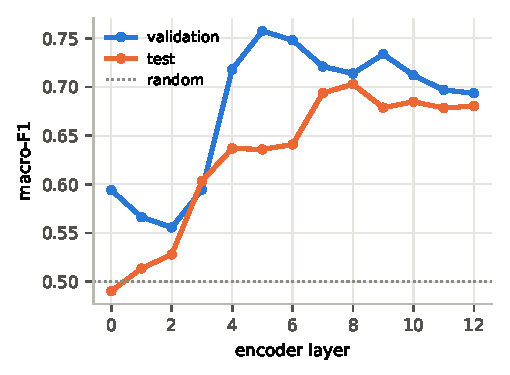
\includegraphics[width=0.42\linewidth]{../figures/fig_layers.pdf}
\caption{Zero-shot macro-F1 by encoder layer. Sense information peaks in the
middle layers. The last layers are shaped by the encoder's own training
objective.}
\label{fig:layers}
\end{figure}

\subsection{Agreement between relatedness models}
\label{sec:agreement}

DURel's Table~3 reports pairwise Spearman correlations between annotators, and
each annotator against the average of the others. Table~\ref{tab:agreement} is
the same table with models in place of annotators, computed on the gold-labelled
COMPARE pairs. Three things stand out.

First, the unsupervised contextual models agree with each other much more than
they agree with people: up to $\rho=0.84$ between adjacent layers, against
$\rho\leq0.36$ with the human labels. The German study shows the opposite
pattern, with an average pairwise $\rho$ of $0.66$ between its five annotators.
A large part of the agreement between our models comes from shared architecture,
not from shared understanding of the words.

Second, supervision shifts the picture in one direction only. The fine-tuned
cross-encoder is by far the closest to the human labels ($\rho=0.58$) but
correlates only weakly with the unsupervised scores ($0.19$ to $0.29$): it has
learnt a decision boundary rather than a relatedness ordering, which is useful
for classification and less useful for graded annotation. The similarity
regression sits in between ($\rho=0.39$ with gold, $0.62$ to $0.64$ with the
layer cosines) and is the better choice when the analysis needs graded scores.
Third, the lexical control is uncorrelated with the gold labels ($-0.02$), the
check that the relatedness signal really is contextual.

\begin{table}[t]\centering\footnotesize
\caption{Spearman correlations between relatedness models and the human labels on
COMPARE pairs (DURel Table~3 analogue). The last row gives each model against the
average of the other models.}
\label{tab:agreement}
\begin{tabular}{lrrrrrrrr}
\toprule
 & cos L5 & cos L8 & cos L12 & sent.\ cos & Jaccard & sim.\ log.\ reg. & fine-tuned CE & \textsc{gold} \\
\midrule
cos L5 & -- & \phantom{$-$}0.76 & \phantom{$-$}0.61 & \phantom{$-$}0.16 & \phantom{$-$}0.19 & \phantom{$-$}0.64 & \phantom{$-$}0.19 & \phantom{$-$}0.33 \\
cos L8 &  & -- & \phantom{$-$}0.84 & \phantom{$-$}0.21 & \phantom{$-$}0.10 & \phantom{$-$}0.62 & \phantom{$-$}0.24 & \phantom{$-$}0.36 \\
cos L12 &  &  & -- & \phantom{$-$}0.27 & $-$0.00 & \phantom{$-$}0.44 & \phantom{$-$}0.29 & \phantom{$-$}0.30 \\
sent.\ cos &  &  &  & -- & $-$0.25 & \phantom{$-$}0.49 & \phantom{$-$}0.24 & \phantom{$-$}0.18 \\
Jaccard &  &  &  &  & -- & $-$0.13 & $-$0.18 & $-$0.02 \\
sim.\ log.\ reg. &  &  &  &  &  & -- & \phantom{$-$}0.29 & \phantom{$-$}0.39 \\
fine-tuned CE &  &  &  &  &  &  & -- & \phantom{$-$}0.58 \\
\textsc{gold} &  &  &  &  &  &  &  & -- \\
\midrule
vs.\ avg.\ of others & \phantom{$-$}0.63 & \phantom{$-$}0.71 & \phantom{$-$}0.64 & \phantom{$-$}0.36 & $-$0.09 & \phantom{$-$}0.61 & \phantom{$-$}0.31 & -- \\
\bottomrule
\end{tabular}
\end{table}

\subsection{Word-level change}
\label{sec:wordlevel}

Figure~\ref{fig:delta} ranks all \numWords{} target words by $\Delta$LATER next
to the human change rate, that is, the share of a word's COMPARE pairs labelled
\emph{different meaning}. The German study found a clear three-way split into
reductive ($>0$), innovative ($<0$) and stable ($\approx 0$) words. Our
distribution is strongly asymmetric: \nReductive{} of \numWords{} words have a
positive $\Delta$LATER. Read literally, that would mean almost every target word
lost a meaning between 2019 and 2021, which is not plausible.

The cause is the corpus effect that \citet{schlechtweg2018durel} warn about.
TempoWiC's later period is 2020--2021, and the target words include
\textit{mask}, \textit{virus}, \textit{delta}, \textit{containment},
\textit{epicenter} and \textit{ventilator}. In those years the words are used in
one pandemic-related way most of the time, so later uses resemble each other
more than earlier ones did and $\mathrm{Mean}_l$ goes up. DURel reads that extra
within-period homogeneity as meaning loss, when what changed is topic
prevalence. This is the main lesson of the transfer: $\Delta$LATER assumes a
corpus that is balanced across periods, and a Twitter sample spanning 2020 is
not.

\begin{figure*}[t]\centering
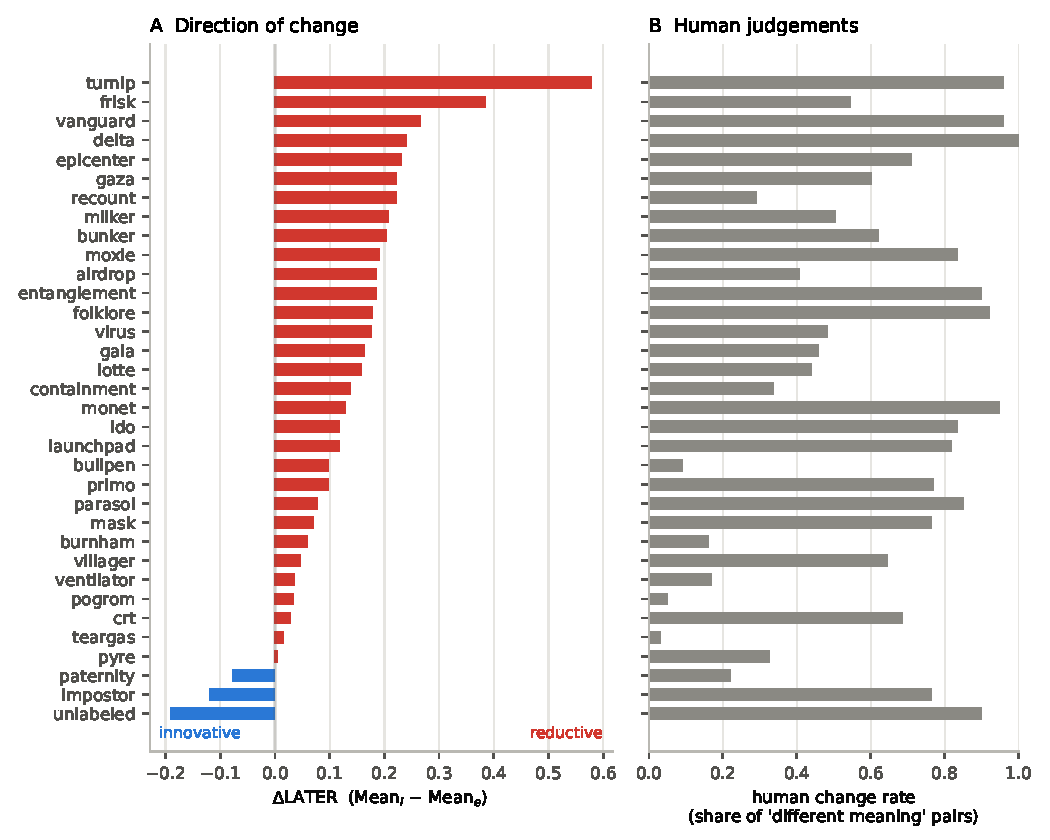
\includegraphics[width=0.60\linewidth]{../figures/fig_delta_later.pdf}
\caption{Target words ranked by $\Delta$LATER (panel A) next to the human change
rate (panel B). The framework reads a positive $\Delta$LATER as reductive change.
Here it mostly reflects pandemic-driven concentration of usage in the later
period.}
\label{fig:delta}
\end{figure*}

\subsection{Do the measures track human judgements?}
\label{sec:measures}

The German study could only validate its measures qualitatively, against what
the historical literature says about each word. TempoWiC lets us do it with
numbers, because each word's human change rate is an independent measurement of
how much it changed. Table~\ref{tab:measures} correlates that rate with each
DURel measure.

COMPARE behaves as the framework predicts. A low COMPARE value means strong
change, and the correlation is $\rho=\rhoCompare{}$ ($p=\rhoCompareP{}$) for the
model our selection protocol picks, namely \mainModel{} with the best validation
macro-F1 (Figure~\ref{fig:scatter}, left). This does not depend on that choice.
Every contextual model lands between $-0.35$ and $-0.68$, the supervised
similarity model is the strongest at $\rho=-0.68$, and the lexical control shows
no relationship at all.

$\Delta$LATER is only weakly related to the human change rate
($\rho=\rhoDeltaLater$) and is insignificant for several models, which matches
\S\ref{sec:wordlevel}. The polysemy-normalised $\Delta$COMPARE, proposed in the
original paper as a refinement, does not improve on plain COMPARE here
($\rho=\rhoDeltaCompare$). Subtracting $\mathrm{Mean}_e$ removes real signal,
because in a one-year Twitter window the earlier-period spread of a word is
driven by topical variety rather than by stable polysemy.

\begin{table}[t]\centering\small
\caption{Spearman correlation of each DURel measure with the human change rate
across \numWords{} words. $^{*}p<0.05$, $^{**}p<0.01$. COMPARE is expected to
correlate negatively.}
\label{tab:measures}
\begin{tabular}{lrrr}
\toprule
Relatedness model & COMPARE & $\Delta$COMPARE & $\Delta$LATER \\
\midrule
cos L5 & $-$0.61$^{**}$ & $-$0.23\phantom{$^{**}$} & \phantom{$-$}0.34$^{*}$\phantom{$^{*}$} \\
cos L8 & $-$0.62$^{**}$ & $-$0.23\phantom{$^{**}$} & \phantom{$-$}0.22\phantom{$^{**}$} \\
cos L12 & $-$0.41$^{*}$\phantom{$^{*}$} & $-$0.19\phantom{$^{**}$} & \phantom{$-$}0.14\phantom{$^{**}$} \\
sim.\ log.\ reg. & $-$0.68$^{**}$ & $-$0.17\phantom{$^{**}$} & \phantom{$-$}0.26\phantom{$^{**}$} \\
fine-tuned CE & $-$0.64$^{**}$ & $-$0.21\phantom{$^{**}$} & $-$0.24\phantom{$^{**}$} \\
sent.\ cos & $-$0.35$^{*}$\phantom{$^{*}$} & $-$0.24\phantom{$^{**}$} & $-$0.06\phantom{$^{**}$} \\
Jaccard & \phantom{$-$}0.15\phantom{$^{**}$} & \phantom{$-$}0.04\phantom{$^{**}$} & \phantom{$-$}0.36$^{*}$\phantom{$^{*}$} \\
\bottomrule
\end{tabular}
\end{table}

\begin{figure}[t]\centering
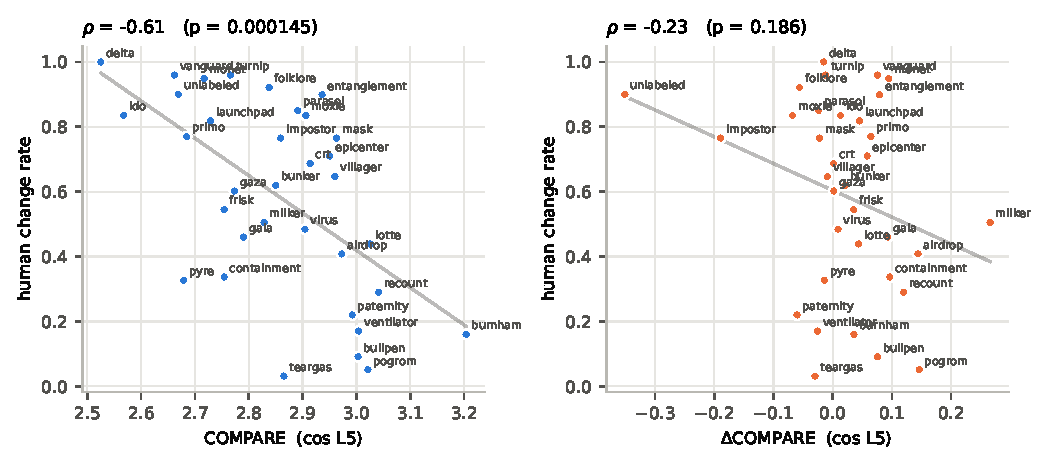
\includegraphics[width=0.70\linewidth]{../figures/fig_compare_scatter.pdf}
\caption{Word-level measures against the human change rate.}
\label{fig:scatter}
\end{figure}

\subsection{Qualitative analysis}

Figure~\ref{fig:dist} contrasts the most stable and the most changed target word,
in the same form as DURel's Figure~4: the distribution of relatedness judgements
per group. For \textit{teargas} (human change rate $0.03$) the three
distributions are almost identical, with group means of $2.89$, $2.91$ and
$2.87$. The word is used the same way in both periods and across them. For
\textit{delta} (change rate $1.00$, with the Greek letter and the airline giving
way to the virus variant) the COMPARE distribution shifts towards low
relatedness, $\mathrm{Mean}_c=2.53$, while the LATER distribution is the most
concentrated at high relatedness, $\mathrm{Mean}_l=2.78$, because the 2021 uses
are nearly all the new sense. That is the pattern the framework is built to
show. It also explains why $\Delta$LATER labels this word reductive ($+0.24$)
when a new dominant meaning is what actually arrived.

\begin{figure}[t]\centering
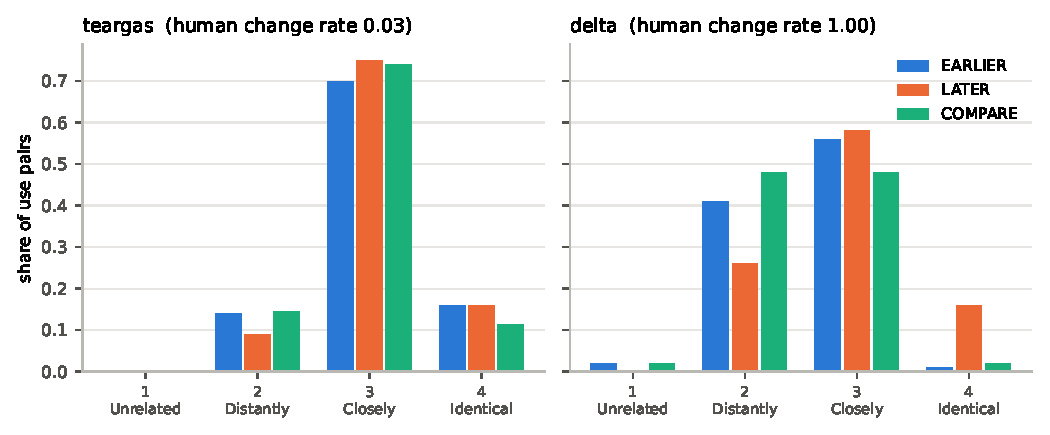
\includegraphics[width=0.70\linewidth]{../figures/fig_group_distributions.pdf}
\caption{Relatedness distributions per group (DURel Figure~4 analogue) for the
most stable and the most changed target word.}
\label{fig:dist}
\end{figure}

\subsection{Where the models fail}
\label{sec:errors}

Table~\ref{tab:worderror} breaks test accuracy down by target word and compares
it against the per-word majority baseline, that is, always predicting the more
frequent label for that word. The picture is sobering: the dev-selected cosine
falls below that baseline on \nBelowMajority{} of the \nTestWords{} test words,
and per-word accuracy is correlated with how skewed the word's labels are
($\rho=\rhoBalanceAcc$, $p=\rhoBalanceAccP$). Words whose pairs are nearly all \emph{different meaning}
(\easiestWord{}, \easiestAcc{}\%) or nearly all \emph{same meaning} are easy;
words with a balanced mix (\hardestWord{}, \hardestAcc{}\%) are hard.

The fine-tuned cross-encoder changes the shape of the errors rather than their
number. It is better on the strongly shifted words and much worse on the stable
ones, because the training words pushed it towards predicting \emph{different
meaning}. The word \textit{burnham} is the clearest case: its pairs are
\emph{same meaning} 84\% of the time, the zero-shot model scores 75.0\% on it,
and the fine-tuned model 21.0\%.

This matters for the DURel measures. Per-pair accuracy is uneven across words,
but the word-level means average over roughly 100 pairs, and COMPARE still
correlates at $\rho=\rhoCompare$ with the human change rate. A measure built on
group means is more robust than the per-pair judgements it is built from, which
is the practical argument for keeping DURel's design when the raters are models.

\begin{table}[t]\centering\footnotesize
\caption{Test accuracy per target word (\%) against the per-word majority
baseline (maj.), sorted by the accuracy of the dev-selected cosine. Every word
has 91--100 test pairs. chg.: human change rate; FT CE: fine-tuned
cross-encoder.}
\label{tab:worderror}
\begin{minipage}[t]{0.49\linewidth}\centering
\begin{tabular}{@{}lrrrr@{}}
\toprule
Word & chg. & maj. & cos L5 & FT CE \\
\midrule
delta & 1.00 & 100.0 & 86.7 & 92.9 \\
unlabeled & 0.90 & 90.0 & 83.0 & 81.0 \\
ido & 0.84 & 83.5 & 82.4 & 83.5 \\
burnham & 0.16 & 84.0 & 75.0 & 21.0 \\
monet & 0.95 & 94.9 & 73.5 & 89.8 \\
moxie & 0.84 & 83.5 & 71.1 & 88.7 \\
vanguard & 0.96 & 96.0 & 69.7 & 91.9 \\
launchpad & 0.82 & 81.8 & 69.7 & 83.8 \\
\bottomrule
\end{tabular}
\end{minipage}\hfill
\begin{minipage}[t]{0.49\linewidth}\centering
\begin{tabular}{@{}lrrrr@{}}
\toprule
Word & chg. & maj. & cos L5 & FT CE \\
\midrule
crt & 0.69 & 68.7 & 68.7 & 68.7 \\
gaza & 0.60 & 60.2 & 67.3 & 62.2 \\
gala & 0.46 & 54.0 & 61.0 & 48.0 \\
milker & 0.51 & 50.5 & 54.5 & 62.6 \\
airdrop & 0.41 & 59.2 & 54.1 & 39.8 \\
pyre & 0.33 & 67.3 & 48.0 & 62.2 \\
bullpen & 0.09 & 90.9 & 42.4 & 80.8 \\
\bottomrule
\end{tabular}
\end{minipage}
\end{table}

\section{Discussion}

\paragraph{What transfers.} Use pairs, the three groups and the relatedness scale
need no language-specific machinery, and COMPARE remains a valid measure of the
degree of change, now with numerical support the original study could not
provide. The claim that DURel is language-independent holds, and extends to
genre: the framework works on 280-character tweets as well as on 19th-century
prose.

\paragraph{What does not.} $\Delta$LATER is fragile. It infers change from the
difference between two within-period means, so any process that changes how
topically concentrated a period is will move it, whether or not a meaning was
gained or lost. A pandemic, an election or a product launch all do this. The
German study meets the same problem in mild form as genre drift in DTA; on
social media it dominates. The original recommendation, a corpus balanced across
periods, is essentially unobtainable for Twitter data spanning 2020.

\paragraph{Models as annotators.} Using models instead of annotators is what
makes this scale: \numTotalPairs{} pairs and no annotation budget. The
substitution is lossy, since models agree with each other far more than with
people, and a benchmark whose splits share no target words additionally
penalises any model that has learnt word-specific associations. At the word
level this matters less than one might expect, because the errors partly average
out over 100 pairs per word and COMPARE still correlates at $\rho=\rhoCompare$.
Per-pair judgements from a model, however, should not be presented as a test
set, and a relatedness model tuned on a handful of words cannot be assumed to
give calibrated relatedness on new ones.

\paragraph{A checklist for modern corpora.} Report COMPARE as the primary
measure and treat $\Delta$LATER as a diagnostic, not as evidence of a change
type. Check the corpus for events that concentrate usage before reading anything
into $\Delta$LATER; plotting $\mathrm{Mean}_e$ and $\mathrm{Mean}_l$ separately,
as in Table~\ref{tab:words}, exposes such an effect at once. And if models do the
rating, prefer one that produces graded scores over one fine-tuned for a binary
decision, since the measures are means and a saturated probability carries no
gradation.

\paragraph{Limitations.} No time-specific encoder was available offline, so the
absolute task numbers sit below published systems; EARLIER and LATER pairs have
no human labels, so only COMPARE means can be checked against people;
\numWords{} words is more than DURel's 22 but still small for correlation
analysis; and CPU-only training limited model size and the hyper-parameter
search.

\section{Conclusion}

We moved DURel from German historical prose to English social media by rebuilding
its three-group design on top of TempoWiC and replacing human annotators with
relatedness models. COMPARE survives the transfer and is validated numerically
against independent human judgements of change ($\rho=\rhoCompare$).
$\Delta$LATER does not survive it: on a corpus spanning 2020 it mostly measures
how far a word's usage narrowed onto one topic. For anyone applying DURel to
contemporary corpora, the practical recommendation is to report COMPARE as the
primary measure and to treat $\Delta$LATER as a diagnostic that is only reliable
when the corpus is balanced across periods.

Three extensions follow naturally. The obvious one is to run the same pipeline
with a time-specific encoder, since TimeLMs is exactly the kind of model the
framework would benefit from and was only unavailable here for environmental
reasons. The second is to replace group means with the Word Usage Graph
machinery of \citet{schlechtweg2021dwug}, which clusters uses instead of
averaging over pairs and would be less sensitive to the topic-concentration
effect of \S\ref{sec:wordlevel}. The third is a small human annotation of
EARLIER and LATER pairs, which would turn the model-based within-period means
into measured ones and make the whole three-group design checkable against
people rather than only its COMPARE part.

{\footnotesize\setlength{\columnsep}{16pt}\begin{multicols}{2}
\bibliography{refs}
\end{multicols}}
\appendix
\section{Per-word measures}
\begin{table}[h]\centering\scriptsize
\caption{Per-word DURel measures. Sp.: TempoWiC split (tr/va/te). chg.\ rate:
share of COMPARE pairs labelled \emph{different meaning} by human annotators.}
\label{tab:words}
\begin{minipage}[t]{0.49\linewidth}\centering
\begin{tabular}{@{}llrrrrrr@{}}
\toprule
Word & Sp. & chg. & Mean$_e$ & Mean$_l$ & Mean$_c$ & $\Delta$L & $\Delta$C \\
\midrule
delta & te & 1.00 & 2.54 & 2.78 & 2.53 & $+$0.24 & $-$0.02 \\
ido & te & 0.84 & 2.55 & 2.67 & 2.57 & $+$0.12 & $+$0.01 \\
vanguard & te & 0.96 & 2.59 & 2.85 & 2.66 & $+$0.27 & $+$0.08 \\
unlabeled & te & 0.90 & 3.02 & 2.83 & 2.67 & $-$0.19 & $-$0.35 \\
pyre & te & 0.33 & 2.69 & 2.70 & 2.68 & $+$0.00 & $-$0.01 \\
primo & va & 0.77 & 2.62 & 2.72 & 2.68 & $+$0.10 & $+$0.06 \\
monet & te & 0.95 & 2.62 & 2.75 & 2.72 & $+$0.13 & $+$0.09 \\
launchpad & te & 0.82 & 2.68 & 2.80 & 2.73 & $+$0.12 & $+$0.05 \\
containment & tr & 0.34 & 2.66 & 2.80 & 2.75 & $+$0.14 & $+$0.10 \\
frisk & tr & 0.54 & 2.72 & 3.10 & 2.75 & $+$0.38 & $+$0.04 \\
turnip & tr & 0.96 & 2.78 & 3.36 & 2.77 & $+$0.58 & $-$0.01 \\
gaza & te & 0.60 & 2.77 & 2.99 & 2.77 & $+$0.22 & $+$0.00 \\
gala & te & 0.46 & 2.70 & 2.86 & 2.79 & $+$0.16 & $+$0.09 \\
milker & te & 0.51 & 2.56 & 2.77 & 2.83 & $+$0.21 & $+$0.27 \\
folklore & tr & 0.92 & 2.89 & 3.07 & 2.84 & $+$0.18 & $-$0.06 \\
bunker & tr & 0.62 & 2.83 & 3.03 & 2.85 & $+$0.20 & $+$0.02 \\
impostor & va & 0.77 & 3.05 & 2.93 & 2.86 & $-$0.12 & $-$0.19 \\
\bottomrule
\end{tabular}
\end{minipage}\hfill
\begin{minipage}[t]{0.49\linewidth}\centering
\begin{tabular}{@{}llrrrrrr@{}}
\toprule
Word & Sp. & chg. & Mean$_e$ & Mean$_l$ & Mean$_c$ & $\Delta$L & $\Delta$C \\
\midrule
teargas & tr & 0.03 & 2.89 & 2.91 & 2.87 & $+$0.02 & $-$0.03 \\
parasol & tr & 0.85 & 2.91 & 2.99 & 2.89 & $+$0.08 & $-$0.02 \\
virus & tr & 0.48 & 2.90 & 3.07 & 2.90 & $+$0.18 & $+$0.01 \\
moxie & te & 0.84 & 2.97 & 3.17 & 2.91 & $+$0.19 & $-$0.07 \\
crt & te & 0.69 & 2.91 & 2.94 & 2.91 & $+$0.03 & $+$0.00 \\
entanglement & tr & 0.90 & 2.86 & 3.04 & 2.94 & $+$0.19 & $+$0.08 \\
epicenter & tr & 0.71 & 2.89 & 3.12 & 2.95 & $+$0.23 & $+$0.06 \\
villager & tr & 0.65 & 2.97 & 3.02 & 2.96 & $+$0.05 & $-$0.01 \\
mask & tr & 0.77 & 2.99 & 3.06 & 2.96 & $+$0.07 & $-$0.02 \\
airdrop & te & 0.41 & 2.83 & 3.01 & 2.97 & $+$0.19 & $+$0.14 \\
paternity & tr & 0.22 & 3.05 & 2.97 & 2.99 & $-$0.08 & $-$0.06 \\
bullpen & te & 0.09 & 2.93 & 3.03 & 3.00 & $+$0.10 & $+$0.08 \\
ventilator & tr & 0.17 & 3.03 & 3.07 & 3.00 & $+$0.04 & $-$0.03 \\
pogrom & tr & 0.05 & 2.88 & 2.91 & 3.02 & $+$0.03 & $+$0.15 \\
lotte & va & 0.44 & 2.98 & 3.14 & 3.03 & $+$0.16 & $+$0.04 \\
recount & va & 0.29 & 2.92 & 3.14 & 3.04 & $+$0.22 & $+$0.12 \\
burnham & te & 0.16 & 3.17 & 3.23 & 3.20 & $+$0.06 & $+$0.04 \\
\bottomrule
\end{tabular}
\end{minipage}
\end{table}

\section{Reproduction}

\paragraph{Pipeline.} The scripts run in this order, each writing into
\texttt{results/}: \texttt{data\_prep.py} (builds the three groups),
\texttt{extract\_encoder.py} (converts the encoder), \texttt{encode.py} (target
vectors at 13 layers), \texttt{zeroshot.py} and \texttt{simlr.py} (unsupervised
scores and the similarity regression), \texttt{finetune.py} and
\texttt{score\_all.py} (cross-encoder), \texttt{durel.py} (measures and
agreement), \texttt{figures.py} and \texttt{make\_tables.py}, and
\texttt{verify.py}.

\paragraph{Verification and provenance.} \texttt{verify.py} recomputes the
headline numbers with a second implementation: macro-F1 by hand rather than with
\texttt{scikit-learn}, the group means from \texttt{pairs.jsonl} rather than from
the pipeline's data frames, and the structural properties of \S\ref{sec:groups}
re-checked. It also compares the numbers quoted in this report against the result
files; all 42 checks pass. Every number here is generated into \texttt{results/}
and \texttt{report/tables/} and read in through \texttt{\textbackslash input}.
\texttt{use\_vectors.npz} (261~MB) is left out of the archive and is regenerated
by \texttt{extract\_encoder.py} and \texttt{encode.py}, which need the spaCy
package \texttt{en\_core\_web\_trf} 3.7.3.

\end{document}
